% !TEX root = main.tex
\documentclass[a4paper, oneside]{article}
\usepackage[utf8]{inputenc}
\usepackage[ngerman]{babel}
\usepackage[top=2.5cm, bottom=3cm, outer=2.5cm, inner=2.5cm, heightrounded]{geometry}
\usepackage{graphicx}
\usepackage{morefloats}
\usepackage{wrapfig}
\usepackage{hyperref}
\usepackage{cite}
\usepackage{siunitx}
\usepackage[default]{sourcesanspro}
\usepackage[T1]{fontenc}
\usepackage{url}
\usepackage{marginnote}
\usepackage[font=footnotesize]{caption}
\usepackage{color}
\usepackage{xcolor}
\usepackage{multicol}
\usepackage[fleqn]{mathtools}
\usepackage{amssymb}
\usepackage{wrapfig}
\usepackage[noindentafter]{titlesec}
\usepackage{fancyhdr}
\usepackage{lastpage}
\usepackage{comment}

%% LÖSUNGEN ANZEIGEN
\newif\ifshow
%\showtrue
\showfalse

%%%SECTIONING
\renewcommand*{\marginfont}{\noindent\rule{0pt}{0.7\baselineskip}\footnotesize}

\newcommand{\aufgabe}[1]{\subsection{#1}}
\newcommand{\loesung}[1]{\subsubsection{#1}}

\newcommand{\simpleset}[1]{\ensuremath \left\{ #1 \right\}}
\newcommand{\ematrix}[2]{\renewcommand{\arraystretch}{1}\ensuremath\left(\begin{array}{@{}#1@{}}#2\end{array}\right)}

\renewcommand{\theenumi}{\alph{enumi})}
\renewcommand{\labelenumi}{\text{\theenumi}}

\newcounter{aufgabe}
%\newenvironment{lsg}{\loesung}{}
\ifshow
  \newenvironment{lsg}{\loesung}{}
\else
  \excludecomment{lsg}
\fi

\newenvironment{inhalt}
  {\paragraph{Inhalt des Übungsblatts:}\itemize\let\origitem\item}
  {\enditemize\vspace{2em}}

\newcommand{\R}{\ensuremath\mathbb{R}}
\newcommand{\N}{\ensuremath\mathbb{N}}
\newcommand{\Z}{\ensuremath\mathbb{Z}}
\newcommand{\LM}{\ensuremath\mathbb{L}}
\newcommand{\intd}{\ensuremath\mathrm{d}}
\newcommand{\e}{\ensuremath\mathrm{e}}
\renewcommand{\d}{\,\mathrm{d}}
\newcommand{\stf}[1]{\ensuremath \left[ #1 \right]}

\newcommand{\cas}{\hfill (CAS)}
\newcommand{\seite}[1]{\textit{(S. #1)}}

\newcommand{\vektor}[1]{\ensuremath\begin{pmatrix} #1 \end{pmatrix}}


\everymath{\displaystyle}

%Malpunkte
\mathcode`\*="8000
{\catcode`\*\active\gdef*{\cdot}}

%SECTION
\titleformat{\section}
{\clearpage\setcounter{aufgabe}{0}\vspace{1em}\Large\raggedright\bfseries}
{}
{0pt}
{}

\titleformat{\subsection}[runin]
{\stepcounter{aufgabe}\vspace{1px}\normalfont\raggedright\bfseries}
{A\theaufgabe: }
{0pt}
{\ }

\titleformat{\subsubsection}[runin]
{\normalfont\raggedright\bfseries}
{Lösung \theaufgabe: }
{0pt}
{\ }


%FANCYHDR
\pagestyle{fancy}
\lhead{\small Simon König\\ Joshua Fabian}
\rhead{\small Mathecrashkurs 2018}
\cfoot{Seite \thepage\thinspace von\thinspace\pageref{LastPage}}
\lfoot{}
\renewcommand{\headrulewidth}{0.5pt}
\renewcommand{\footrulewidth}{0pt}

\title{Mathe-Crashkurs 2018 - Übungsblatt}
\date{\today}
\author{Simon König, Joshua Fabian}


\chead{\Large Übungsblatt 0}
\begin{document}

\begin{inhalt}
  \item Gleichungen \seite{7}
  \item Monotonie, Achsenschnittpunkte \seite{13}, Trigonometrie \seite{16}
	\item Ableiten \seite{23}
	\item Tangenten, Normalen \seite{22}
\end{inhalt}



\aufgabe{Gleichungen:} Löse die Gleichungen für $x\in \R$
\begin{multicols}{2}
  \begin{enumerate}
    \item $3x + 5 = 23$
    \item $8x - 12 = 28$
    \item $7x + 3 = 5x + 12$
		\item $17-4x=1-12x$
    \item $4(9x - 11) - 12(3x - 4) = 4$
    \item $\frac{x+2}{3} + \frac{x-1}{15} = \frac{2x+3}{5}$
		\item $(x-5)^2=(x-3)(x+3)$
  \end{enumerate}
\end{multicols}

\begin{lsg}{}
  \begin{multicols}{2}
	  \begin{enumerate}
      \item $3x = 18 \rightsquigarrow x = 6$
      \item $8x = 40 \rightsquigarrow x = 5$
      \item $2x = 9 \rightsquigarrow x = 4,5$
			\item \begin{align*}
				17-4x &= 1-12x\\
				16 &= 8x\\
				x &= 2
			\end{align*}
      \item Ausmultiplizieren, die Gleichung gilt für alle $x$.
      \item \begin{align*}
        \frac{5x+10}{15} + \frac{x-1}{15} &= \frac{2x+3}{5}\\
        \frac{6x+9}{15} &= \frac{2x+3}{5}\\
        \frac{2x+3}{5} &= \frac{2x+3}{5}\\
        \rightsquigarrow \text{ gilt für alle }x&
      \end{align*}
			\item \begin{align*}
				(x-5)^2 &= (x-3)(x+3)\\
				x^2-10x+25 &= x^2+9\\
				10x &= 16\\
				x &= 1,6
			\end{align*}
    \end{enumerate}
  \end{multicols}
\end{lsg}

\aufgabe{Mitternachtsformel:} Löse die Gleichungen für $x\in \R$ mithilfe der Mitternachtsformel
\begin{multicols}{3}
  \begin{enumerate}
    \item $x^2 - 10x + 24 = 0$
    \item $x^2 + 6x - 16 = 0$
    \item $x^2 - 9x = 22$
    \item $x^2 = 3x + 18$
    \item $\frac{x(x-10)}{2} = 12$
  \end{enumerate}
\end{multicols}

\begin{lsg}{}
  \begin{equation*}
    \text{für das Polynom $ax^2+bx+c=0$ gilt für die Nullstellen: } x_{1,2}=\frac{-b\pm\sqrt{b^2-4ac}}{2a}
  \end{equation*}
    \begin{enumerate}
      \item \begin{align*}
      x_{1,2}&=\frac{10\pm\sqrt{(-10)^2-4*1*24}}{2}\\
      &=\frac{10\pm\sqrt{100-96}}{2}\\
      &=\frac{10\pm2}{2}\\
      \rightarrow x_1&=6\\
      \rightarrow x_2&=4\\
      \end{align*}
      \item \begin{align*}
      x_{1,2}&=\frac{-6\pm\sqrt{6^2-4*1*(-16)}}{2}\\
      &=\frac{-6\pm\sqrt{36+64}}{2}\\
      &=\frac{-6\pm10}{2}\\
      \rightarrow x_1&=4\\
      \rightarrow x_2&=-16\\
      \end{align*}
      \item
      \begin{align*}
        &x^2 - 9x = 22 \Leftrightarrow x^2 - 9x - 22 = 0\\
        x_{1,2}&=\frac{9\pm\sqrt{(-9)^2-4*1*(-22)}}{2}\\
        &=\frac{9\pm\sqrt{81+88}}{2}\\
        &=\frac{9\pm\sqrt{169}}{2}\\
        &=\frac{9\pm13}{2}\\
        \rightarrow x_1&=6\\
        \rightarrow x_2&=-2\\
      \end{align*}
      \item
      \begin{align*}
        &x^2 = 3x + 18 \Leftrightarrow x^2 - 3x - 18 = 0\\
        x_{1,2}&=\frac{3\pm\sqrt{(-3)^2-4*1*(-18)}}{2}\\
        &=\frac{3\pm\sqrt{9+72}}{2}\\
        &=\frac{3\pm\sqrt{91}}{2}\\
        &=\frac{3\pm9}{2}\\
        \rightarrow x_1&=6\\
        \rightarrow x_2&=-3\\
      \end{align*}
      \item
      \begin{align*}
        &\frac{x(x-10)}{2} = 12 \Leftrightarrow x(x-10)=24 \Leftrightarrow x^2 - 10x - 24 = 0\\
        x_{1,2}&=\frac{10\pm\sqrt{(-10)^2-4*1*(-24)}}{2}\\
        &=\frac{10\pm\sqrt{100+96}}{2}\\
        &=\frac{10\pm\sqrt{196}}{2}\\
        &=\frac{10\pm14}{2}\\
        \rightarrow x_1&=12\\
        \rightarrow x_2&=-2\\
      \end{align*}
    \end{enumerate}
\end{lsg}


\aufgabe{Wurzeln: } Vereinfache so weit möglich
\begin{multicols}{3}
  \begin{enumerate}
    \item $4\sqrt{7}-6\sqrt{7} + 3\sqrt{7}$
    \item $\sqrt{180}$
    \item $\sqrt{192x^5}$
    \item $\sqrt{\frac{80x^2}{147}}$
    \item $\sqrt{3}\cdot\sqrt{300}$
    \item $\sqrt{27}-\sqrt{25}-\sqrt{3}$
  \end{enumerate}
\end{multicols}

\begin{lsg}{}
  \begin{multicols}{3}
    \begin{enumerate}
      \item $\sqrt{7}$
      \item $\sqrt{4*45}=2*\sqrt{5*9}=6*\sqrt 5$
      \item $\sqrt{192*x^5}=\sqrt{192}*\sqrt{x^5}=\sqrt{2*96}*\sqrt{x^2*x^2*x}=4*x^2*\sqrt{12x}$
      \item $\frac{\sqrt{80x^2}}{\sqrt{147}} = \frac{4x*\sqrt{5}}{7*\sqrt{3}}$
      \item $\sqrt{3}*\sqrt{300}=3*\sqrt{100}=30$
      \item $\sqrt{3*9}-5-\sqrt{3}=3*\sqrt{3}-5-\sqrt{3}=2*\sqrt{3}-5$
    \end{enumerate}
  \end{multicols}
\end{lsg}


\aufgabe{Satz vom Nullprodukt: } Löse die Gleichungen für $x\in \R$ mit dem Satz vom Nullprodukt
\begin{multicols}{3}
  \begin{enumerate}
		\item $\sin(x)*(\cos(x)-2)=0$\\ $\text{ mit }(0\leq x<2\pi)$\columnbreak
		\item $\sin^2(x)-2\sin(x) = 0$\\ $\text{ mit }(0\leq x<2\pi)$\columnbreak
    \item $x^3 - 4x = 0$
    \item $3x^3-6x^2=0$
  \end{enumerate}
\end{multicols}

\begin{lsg}{}
  \begin{enumerate}
		\item $\cos(x)-2 < 0$ für alle $x\in \R \quad\rightsquigarrow \sin(x)=0 \Leftrightarrow x=k*\pi, k\in\Z$
    \item $x(x^2-4) = 0 \rightsquigarrow x_1=0, x_2=2, x_3=-2$
    \item $\sin(x)*(\sin(x)-2) = 0 \rightsquigarrow x_1=0, x_2=\pi$
    \item $x^2(3x-6)=0 \rightsquigarrow x_1=0, x_2=2$
  \end{enumerate}
\end{lsg}



\aufgabe{Substitution:} Löse die Gleichungen - ohne CAS
\begin{multicols}{3}
  \begin{enumerate}
    \item $2x^4 - 5x^2 + 2 = 0$
    \item $x^4 - 4x^2 + 3 = 0$
    \item $\sin(3x) = 1 (0\leq x \leq 2\pi)$
    \item $\sin^2(2x) + 2\sin(2x) = -1 \\(0\leq x \leq 2\pi)$
    \item $e^{2x} - e^x = 0$
		\item $\cos^2(x)-3\cos(x)+2=0 \\(0\leq x \leq 2\pi)$
  \end{enumerate}
\end{multicols}

\begin{lsg}{}
	\begin{enumerate}
    \item Mit Substitution $x^2=u$:

		$u_1=\frac 1 2, u_2=2$.

		Resubstitution:

		$u_1=\frac 1 2 = x^2 \rightsquigarrow x=\frac 1{\sqrt 2},  u_2=2 = x^2 \rightsquigarrow x=\sqrt 2$
    \item Mit Substitution $x^2=u$:

		$u_1=1, u_2=3$.

		Resubstitution:

		$x_1=1, x_2=\sqrt 3$
    \item $\sin(3x) = 1$
		Mit Substitution $u=3x$:

		$\sin(u)=1 \rightsquigarrow u=k*2\pi+\frac {\pi} 2 \quad k\in\Z$

		Resubstitution:

		$k*2\pi+\frac {\pi} 2 = 3x \rightsquigarrow x=\frac {k*2\pi} 3+\frac {\pi} 6\quad x_1=\frac \pi 6, x_2=\frac {5\pi} 6, x_3=\frac{9\pi} 6$
    \item Mit Substitution $u=\sin(2x)$:

		$u^2 + 2u + 1 = 0$

		Mitternachtsformel: $u_1=-1$

		Resubstitution: $u_1=-1=\sin(2x)$

		mit Substitution $v=2x$ folgt $-1=\sin(v) \rightarrow v=k*2\pi+\frac {3\pi} 2 \quad k\in\Z$

		Resubstitution:

		$v=k*2\pi+\frac {3\pi} 2=2x \rightsquigarrow x=k*\pi+\frac {3\pi} 4 \quad x_1=\frac {3\pi} 4, x_2=\frac {7\pi} 4$
    \item Siehe oben, $x=0$
		\item Siehe oben, $x_1=0,x_2=2\pi$
  \end{enumerate}
\end{lsg}


\aufgabe{Nullstellen von Funktionen: } Bestimme die Nullstellen der Funktionen
\begin{multicols}{3}
  \begin{enumerate}
    \item $f(x) = \frac 1 2 (x-2)^2 -4$
    \item $f(x) = 3x^2-2x+2$
    \item $f(x) = x^4-1$
  \end{enumerate}
\end{multicols}
\begin{lsg}{}
  \begin{multicols}{3}
    \begin{enumerate}
      \item \begin{align*}
        \frac 1 2 (x-2)^2 &= 4\\
        (x-2)^2 &= 8\\
        (x-2)&=\pm\sqrt 8\\
        \rightarrow x_1&=2+\sqrt 8\\
        \rightarrow x_2&=2-\sqrt 8\\
      \end{align*}
      \columnbreak
      \item Mit der Mitternachtsformel: Term unter der Wurzel ist negativ, d.h. keine Lösungen
      \columnbreak
      \item Mit Substitution: $u\coloneqq x^2$, $u_1=1, u_2=-1$

			Resubstitution: $u=x^2 \rightsquigarrow x_1=1, x_2=-1$
    \end{enumerate}
  \end{multicols}
\end{lsg}

\aufgabe{Schnittpunkte von Funktionen: } In welchen Punkten schneiden sich die Funktionen?
\begin{multicols}{3}
  \begin{enumerate}
    \item $f(x) = x^2$, $g(x) = 2x$
    \item $f(x) = \frac 1 2 x^4$, $g(x) = x^2+4$
  \end{enumerate}
\end{multicols}
\begin{lsg}{}
  \begin{multicols}{2}
    \begin{enumerate}
      \item \begin{align*}
        x^2 &= 2x\\
        x^2-2x &= 0\\
        \intertext{Mit der Mitternachtsformel: }
        x_1 &= 0, x_2 =2\\
        \intertext{Bestimmung der Werte der Stellen: }
        f(0) &= 0, f(2) = 4\\
        \LM &= \left\{\ (0|0),(2|4) \ \right\}
      \end{align*}

      \columnbreak
      \item
      \begin{align*}
        \frac 1 2 x^4 &= x^2+4\\
        \frac 1 2 x^4 -x^2 -4 &= 0\\
      \end{align*}
      Substitution $x^2=u$
      \begin{align*}
        \frac 1 2& u^2 -u -4 = 0\\
        u_{1,2}&=\frac{1\pm\sqrt{1-4*0.5*(-4)}}{1}\\
        &= 1\pm\sqrt{9}\\
        u_1 &= 4\quad u_2=-2\\
      \end{align*}
      Resubstitution von $u_1$ ($u_2 < 0 \rightarrow $ nicht reelles Ergebnis):
      \begin{align*}
        x^2=4\\
        x_1 = -2, x_2 = 2\\
        \intertext{Bestimmung der Werte der Stellen: }
        g(-2)=8, g(2)=8\\
        \LM = \left\{\ (-2|8),(2|8) \ \right\}
      \end{align*}
    \end{enumerate}
  \end{multicols}
\end{lsg}


\aufgabe{Trigonometrie: }
	\begin{enumerate}
		\item Beschreiben Sie in Worten, wie sich der Graph von $g(x)=3\sin(3(x+1))-3$ von $\sin(x)$ unterscheidet.
		\item Gib die Amplitude, Verschiebung und Periode der folgenden Sinus-Funktionen an:
		\begin{itemize}
		\item $\sin\left(2(x-2)\right)+1$
		\item $4\sin\left(\frac{3x}{4\pi}\right)$
		\item $-2\sin\left(4x+8\right)-3\pi$
		\end{itemize}
		\item In Abbildung \ref{sinus:fig} gegeben ist der Graph F einer verschobenen Sinusfunktion. Gib einen möglichen Funktionsterm $f(x)$ an.
		\begin{figure}[h]
		\centering
		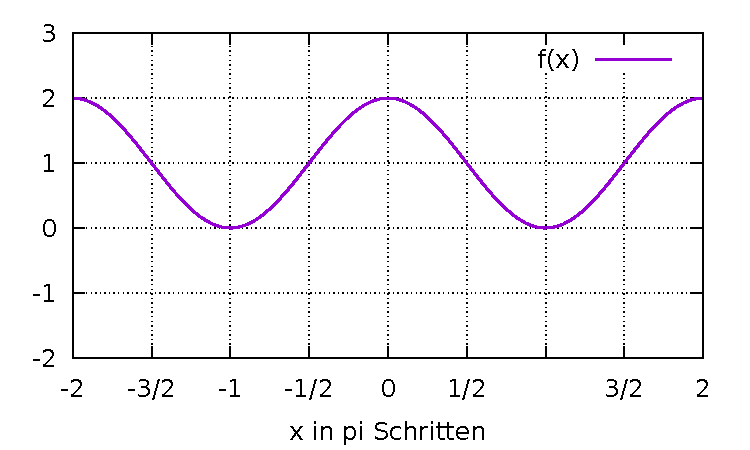
\includegraphics[scale=0.7]{Afg_sinus.pdf}
			\caption{Sinus-Funktion}
			\label{sinus:fig}
		\end{figure}
	\end{enumerate}
\begin{lsg}{}
	\begin{enumerate}
		\item Amplitude 3, Phasenverschiebung um 1 nach links, Verschiebung um 3 nach unten und Änderung der Periode auf $\frac{2\pi}{3}$
		\item \begin{itemize}
			\item Amplitude: $1$, Verschiebung von $(0|0)$ zu $(2|1)$, Periode: $\pi$
			\item Amplitude: $4$, Periode: $\frac{3}{2}$
			\item Amplitude: $2$, Verschiebung von $(0|0)$ zu $(-2|-3\pi)$, Periode: $\frac \pi 2$
		\end{itemize}
		\item Um $1$ vertikal und entweder um $-\frac{\pi}{2}$ oder $\frac{3\pi}{2}$ horizontal verschoben:\\
		$f(x)=\sin\left(x+\frac{1}{2}\pi\right)+1$ oder $f(x)=\sin\left(x-\frac{3\pi}{2}\right)+1$
	\end{enumerate}
	\end{lsg}



\aufgabe{Ableitungen: } Berechne jeweils die erste Ableitung der Funktionen
\begin{multicols}{3}
	\begin{enumerate}
		\item $f(x)=3x^4+2x^3+x^2-10$
	  \item $g(x)=x^2\e^x$
		\item $h(x)=x^x$
	  \item $j(x)=\ln(\e^{3x}\sin(2x))$
		\item $k(x) = 2(3x^2+x)^3$
    \item $l(x) = \frac{4}{(2x+1)^2}$
    \item $m(x) = 2x\sqrt{x^2+1}$
    \item $n(x) = \sqrt{x}\sin(x^2)$
    \item $o(x) = \sqrt{\cos(x)\cdot\sqrt{x+1}}$
    \item $p(x) = \frac{2x+3}{\sin(3x)}$
	\end{enumerate}
\end{multicols}

\begin{lsg}{}
	\begin{multicols}{2}
		\begin{enumerate}
			\item Summenregel: \begin{align*}
			f'(x)=12x^3+6x^2+2x
			\end{align*}
			\item Produktregel: \begin{align*}
			g'(x)=2x\e^x+x^2\e^x
			\end{align*}
			\item Umformung auf handlicheres Format: \begin{align*}
		    h(x)&= x^x= \e^{x\ln(x)}\\
		    \intertext{Ketten- und Produktregel: }
				h'(x)&=\e^{x\ln(x)}* \left(\ln(x)+x*\frac{1}{x}\right) \\
				&= \e^{x\ln(x)}*\ln(x)+1
		  \end{align*}
		  \item Umformung auf handlicheres Format: \begin{align*}
		    j(x)&= \ln(\e^{3x}\sin(2x))\\
				&= \ln(\e^{3x}) + \ln(\sin(2x)) \\
				&= 3x + \ln(\sin(2x))\\
				\intertext{Kettenregel:}
		    j'(x)&=3+\frac{1}{\sin(2x)} * 2*\cos(2x) \\
				&= \frac{2\cos(2x)}{\sin(2x)}+3
		  \end{align*}
			\item $k'(x) = 6(3x^2+x)^2*(6x+1)$
	    \item $l'(x) = -16(2x+1)^{-3}$
	    \item $m'(x) = 2\sqrt{x^2+1}+\frac{2x^2}{\sqrt{x^2+1}}$
	    \item $n'(x) = 2x^{\frac 3 2}*\cos(x^2)+\frac{\sin(x^2)}{2\sqrt x}$
	    \item $o'(x) = \frac{-\sin(x)\sqrt{x+1}}{2*\sqrt{\cos(x)*\sqrt{x+1}}}+\frac{\cos(x)}{4*\sqrt{\cos(x)\sqrt{x+1}}*\sqrt{x+1}}$
	    \item $p'(x) = \frac{-6\left(3x\cos(3x)-\sin(3x)\right)}{\left(\sin(3x)\right)^2}$
		\end{enumerate}
	\end{multicols}
\end{lsg}



\aufgabe{Monotonieuntersuchung: }
\begin{enumerate}
	\item Definiere, wann eine Funktion in einem Intervall als streng monoton steigend bezeichnet wird.
	\item Untersuche die gegebenen Funktionen auf Monotonie und gib Art und Lage der Extrempunkte an:
	\begin{multicols}{2}
		\begin{enumerate}
			\item $f(x)=x^2-4x+5$
			\item $g(x)=x^3-3x^2-24x+6$
			\item $h(x)=3x^4+8x^3-48x^2+3$
			\item $j(x)=\frac{2x^2}{2x-1}$ (Achtung: gebrochenrational)
		\end{enumerate}
	\end{multicols}
\end{enumerate}
\begin{lsg}{}
	\begin{enumerate}
		\item Eine Funktion ist über dem Intervall $[x_0;x_1]$ streng monoton steigend, wenn gilt: $f'(x)>0$ für alle $x_0\leq x \leq x_1$, äquivalent dazu: $\forall a,b\in[x_0;x_1], a<b : f(a)>f(b)$
		\item
		\begin{enumerate}
			\item $f'(x)=2x-4$

			Bestimmen der Nullstellen:
			\begin{equation*}
				f'(x)=0 \rightsquigarrow x_0=2
			\end{equation*}
			Da $f'(x)>0$ für $x>x_0$ gilt:
			\begin{align*}
				f \begin{cases}
					\text{streng monoton fallend für $x<2$}\\
					\text{Tiefpunkt bei $T(2|f(2))=T(2|1)$}\\
					\text{streng monoton steigend für $x>2$}\\
				\end{cases}
			\end{align*}
			\item $g'(x)=3x^2-6x-24$

			Bestimmen der Nullstellen:
			\begin{equation*}
				g'(x)=0=3x^2-6x-24 \rightsquigarrow x_1=-2 ,x_2=4
			\end{equation*}
			Durch Berechnen von zufälligen Funktionswerten in den drei entstehenden Intervallen erhält man:
			\begin{align*}
				g \begin{cases}
					\text{streng monoton steigend für $x<-2$}\\
					\text{Hochpunkt bei $H(-2|f(-2))=H(-2|34)$}\\
					\text{streng monoton fallend für $-2<x<4$}\\
					\text{Tiefpunkt bei $T(4|f(4))=T(4|-74)$}\\
					\text{streng monoton steigend für $x>4$}\\
				\end{cases}
			\end{align*}
			\item $h'(x)=12x^3+24x^2-96x=12x*(x^2+2x-8)$

			Berechnen der Nullstellen mit der Mitternachtsformel und dem Satz vom Nullprodukt:
			\begin{equation*}
				h'(x)=0 \rightsquigarrow x_1=-4, x_2=0, x_3=2
			\end{equation*}
			Durch Berechnen von zufälligen Funktionswerten in den entstehenden Intervallen erhält man:
			\begin{align*}
				h'(x) \begin{cases}
					\text{< 0 für $x<-4$}\\
					\text{> 0 für $-4<x<0$}\\
					\text{< 0 für $0<x<2$}\\
					\text{> 0 für $x>2$}\\
				\end{cases}
			\end{align*}
			Mit Extrempunkten von $h$: $T_1(-4|-509), H(0|3), T_2(2|-77)$
			\item $j'(x)=\frac{4x(x-1)}{(2x-1)^2}$

			Nullstellen der Ableitung sind die Nullstellen des Zählers:
			$4x(x-1)=0 \rightsquigarrow x_1=0, x_2=1$

			$j$ hat eine Polstelle bei der Nullstelle des Nenners:
			$2x-1=0 \rightsquigarrow x_p=\frac 1 2$

			\begin{align*}
				j'(x) \begin{cases}
					\text{> 0 für $x<0$}\\
					\text{< 0 für $0<x<\frac 1 2$}\\
					\text{< 0 für $\frac 1 2<x<1$}\\
					\text{> 0 für $x>1$}\\
				\end{cases}
			\end{align*}

			Mit Extrempunkten von $j$: $H(0|0), T(1|2)$ und einer Polstelle (senkrechte Asymptote) bei $x=\frac 1 2$
		\end{enumerate}
	\end{enumerate}
\end{lsg}



\aufgabe{Tangenten: }
\begin{enumerate}
	\item Gegeben ist die Funktion $g$ mit $\ g(x)=2x^2+1$. Bestimme die Gleichung der Tangente und der Normalen an den Graphen G von $g$ im Punkt $P(1|3)$.
  \item Bestimme die Gleichung der Tangente und Normalen an den Graphen G von $g$ mit der Steigung $1$.
  \item Bestimme die Gleichungen der beiden Tangenten an den Graphen G von $g$, die durch den Punkt $Q(3|17)$ gehen und gib die Berührpunkte der Tangenten mit dem Graphen G von $g$ an.
\end{enumerate}
\begin{lsg}{}
	\begin{align*}
		\text{Tangentengleichung: }  t(x,x_0)&=g'(x_0)*(x-x_0)+g(x_0)\\
	\text{Normalengleichung: }n(x,x_0)&=-\frac{1}{g'(x_0)}*(x-x_0)+g(x_0)
	\end{align*}

	\begin{enumerate}
		\item Aus Punkt P(1/3) folgt: $x_0=1,\ g(x_0)=3$ und ableiten ergibt $\ g'(x)=4x$
		\begin{align*}
		\text{Damit gilt: }\ t(x)&=4*(x-1)+3 \\
		\text{und: }\ n(x)&=-\frac{1}{4}*(x-1)+3
		\end{align*}
		\item \begin{align*}
			\text{Tangentengleichung: }\ g'(x_0)&=1 \rightsquigarrow x_0=\frac{1}{4}\\
			g\left(\frac{1}{4}\right)&=\frac{9}{8}\\
			t(x)&=1*\left(x-\frac{1}{4}\right)+\frac{9}{8}\\
			\text{Normalengleichung:}\ -\frac{1}{g'(x_0)}&=1 \rightsquigarrow x_0=-\frac{1}{4}\\
			g\left(-\frac{1}{4}\right)&=\frac{9}{8}\\
			n(x)&=1*\left(x+\frac{1}{4}\right)+\frac{9}{8}
			\end{align*}
			\item Aus dem Punkt $Q(3|517)$ folgt: $\ t(3)=17$, daher gilt für die Tangentengleichungen:\begin{align*}
			17&=g'(x_0)*(3-x_0)+g(x_0) \rightsquigarrow x_{0,1}=2,\ x_{0,2}=4\\
			t_1(x)&=8*(x-2)+9\\
			t_2(x)&=16*(x-4)+33
			\end{align*}
	\end{enumerate}
\end{lsg}


\end{document}
